\chapter{OpenMPI}

\section{Il Problema della Scalabilità}
Il passaggio al modello a memoria distribuita è dettato da limiti fisici e architetturali.
\begin{itemize}
    \item \textbf{Memoria Condivisa (es. OpenMP)}: Scala efficacemente fino a qualche decina di core sullo stesso nodo. Quando il numero di core necessari supera quelli fisicamente condivisi o il problema diventa troppo grande, questo modello cessa di funzionare.
    \item \textbf{Memoria Distribuita (es. MPI)}: Ogni processo possiede la propria RAM privata. La comunicazione non avviene tramite variabili condivise, ma attraverso lo scambio esplicito di messaggi (\textit{msg}) tra processi indipendenti.
\end{itemize}

\section{Cos'è MPI?}
MPI (\textit{Message Passing Interface}) è lo standard per la programmazione parallela basata sullo scambio esplicito di messaggi tra processi indipendenti. Non è un linguaggio, ma una specifica di interfaccia multi-piattaforma e vendor-neutral.

\vspace{0.5cm}
\noindent
Le caratteristiche principali dello standard sono:
\begin{enumerate}
    \item \textbf{Standard Aperto}: Gestito dall'MPI Forum, che riunisce vendor, centri di ricerca e università.
    \item \textbf{Portabilità Totale}: Lo stesso codice sorgente è eseguibile su diverse architetture, dal singolo laptop ai cluster Linux, fino ai supercomputer più potenti.
    \item \textbf{Evoluzione Continua}: Dalle prime specifiche MPI-1 (1994) alle più recenti MPI-4 (2021), che introducono modelli a sessioni e collettive persistenti.
\end{enumerate}


\begin{framed}
\noindent
\textbf{Il Modello di Esecuzione: SPMD} \\
MPI adotta il paradigma \textbf{SPMD} (\textit{Single Program, Multiple Data}).
\begin{itemize}
    \item \textbf{Binario Unico}: Tutti i processi eseguono lo stesso file eseguibile.
    \item \textbf{Rank}: La distinzione dei ruoli avviene a runtime tramite il \textit{rank}, ovvero l'identificatore numerico unico di ogni processo.
    \item \textbf{Esempio}: In un blocco \texttt{if (rank == 0)}, il processo "root" può decidere di raccogliere i risultati, mentre gli altri processi ("worker") eseguono i calcoli e inviano i dati.
\end{itemize}
\end{framed}

\section{Struttura di un Programma e Comunicatori}
L'esecuzione parallela avviene all'interno di un blocco delimitato da chiamate di inizializzazione e chiusura.
\begin{itemize}
    \item \texttt{MPI\_Init}: Inizializza il runtime; deve essere la prima chiamata MPI.
    \item \texttt{MPI\_Comm\_rank}: Restituisce il rank del processo corrente.
    \item \texttt{MPI\_Comm\_size}: Restituisce il numero totale di processi nel comunicatore.
    \item \texttt{MPI\_Finalize}: Libera le risorse; nessuna chiamata MPI è permessa dopo di essa.
\end{itemize}

\vspace{0.3cm}
\noindent
\textbf{Il Contesto: I Comunicatori} \\
Un comunicatore è un oggetto che racchiude un gruppo di processi e un contesto di comunicazione. Ogni messaggio viaggia all'interno di un comunicatore: due messaggi con lo stesso tag ma su comunicatori diversi non si confondono mai. Questo è il meccanismo fondamentale con cui le librerie MPI proteggono i propri messaggi interni dall'interferenza con i messaggi dell'utente. Il comunicatore predefinito è \texttt{MPI\_COMM\_WORLD}, che include tutti i processi. È possibile creare sotto-comunicatori tramite \texttt{MPI\_Comm\_split}, partizionando i processi in base a un \textit{colore} (gruppo di appartenenza) e una \textit{chiave} (ordinamento interno).

\section{Tipi di Dati e Messaggi}
MPI definisce un insieme di tipi primitivi che corrispondono ai tipi del linguaggio host. Sono usati per specificare il tipo e la quantità dei dati in ogni operazione di comunicazione e per gestire la comunicazione tra architetture diverse.
\begin{itemize}
    \item \textbf{Tipi Primitivi}: Corrispondono ai tipi C (es. \texttt{MPI\_INT}, \texttt{MPI\_DOUBLE}, \texttt{MPI\_CHAR}).
    \item \textbf{Tipi Derivati}: Permettono di descrivere layout di memoria non contigui (strutture, colonne di matrici) senza buffer temporanei.
\end{itemize}

\begin{figure}[H]
    \centering
    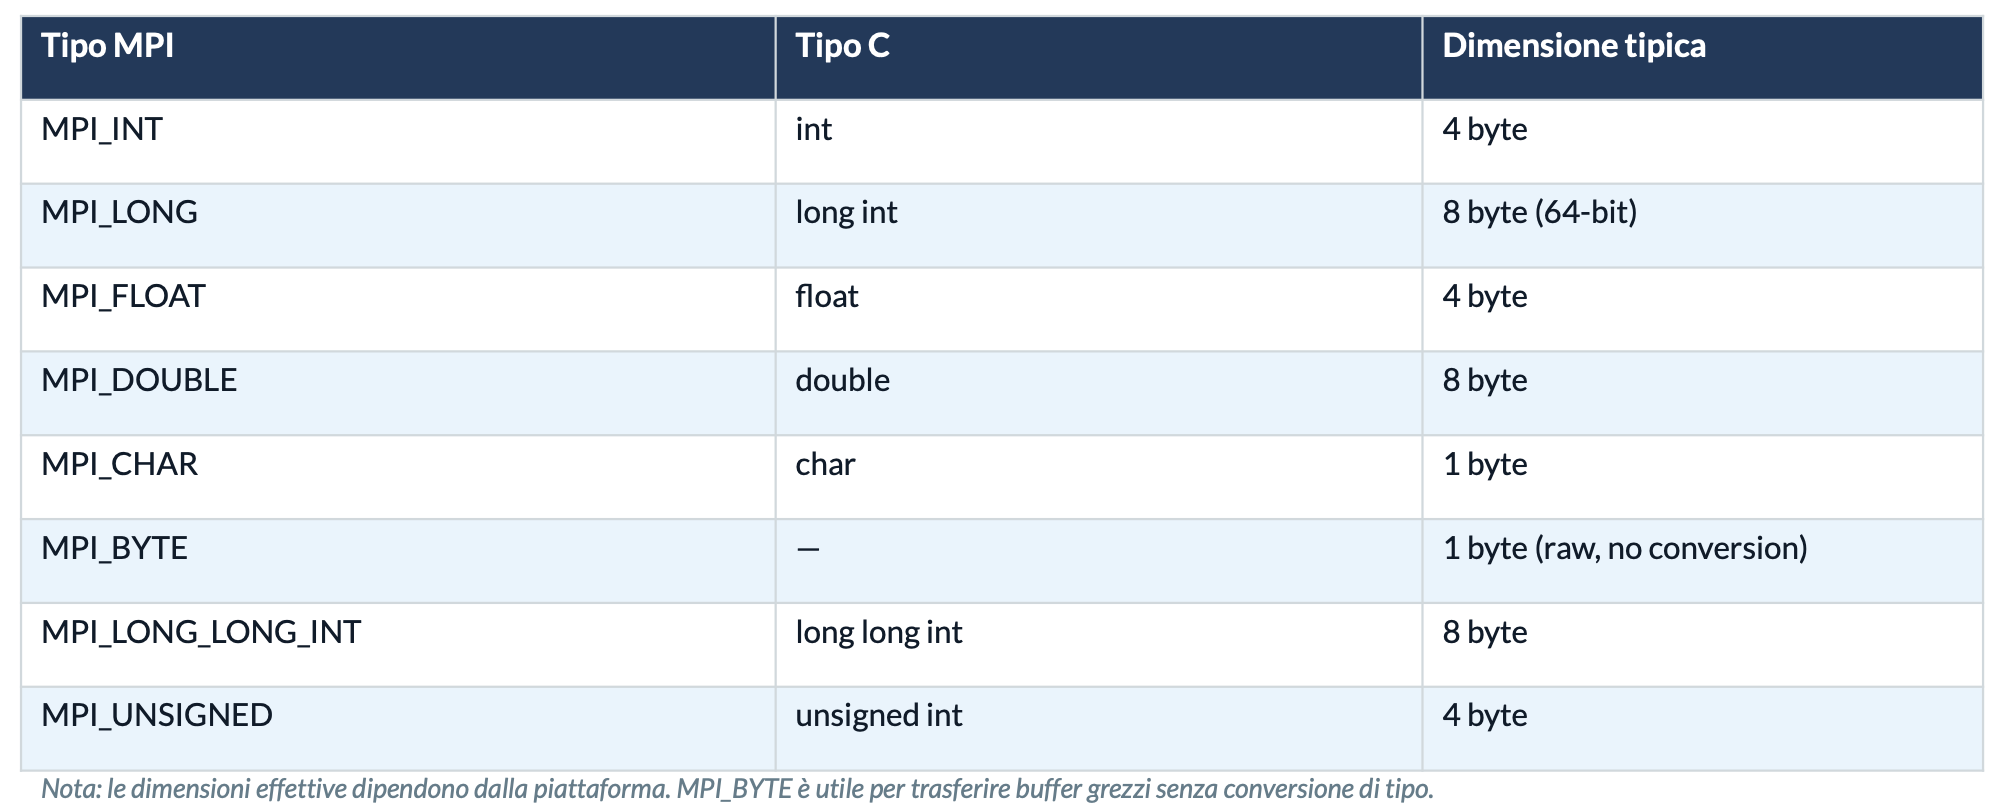
\includegraphics[width=0.9\linewidth]{Images/cap_8/primitivi.png}
\end{figure}

\begin{figure}[H]
    \centering
    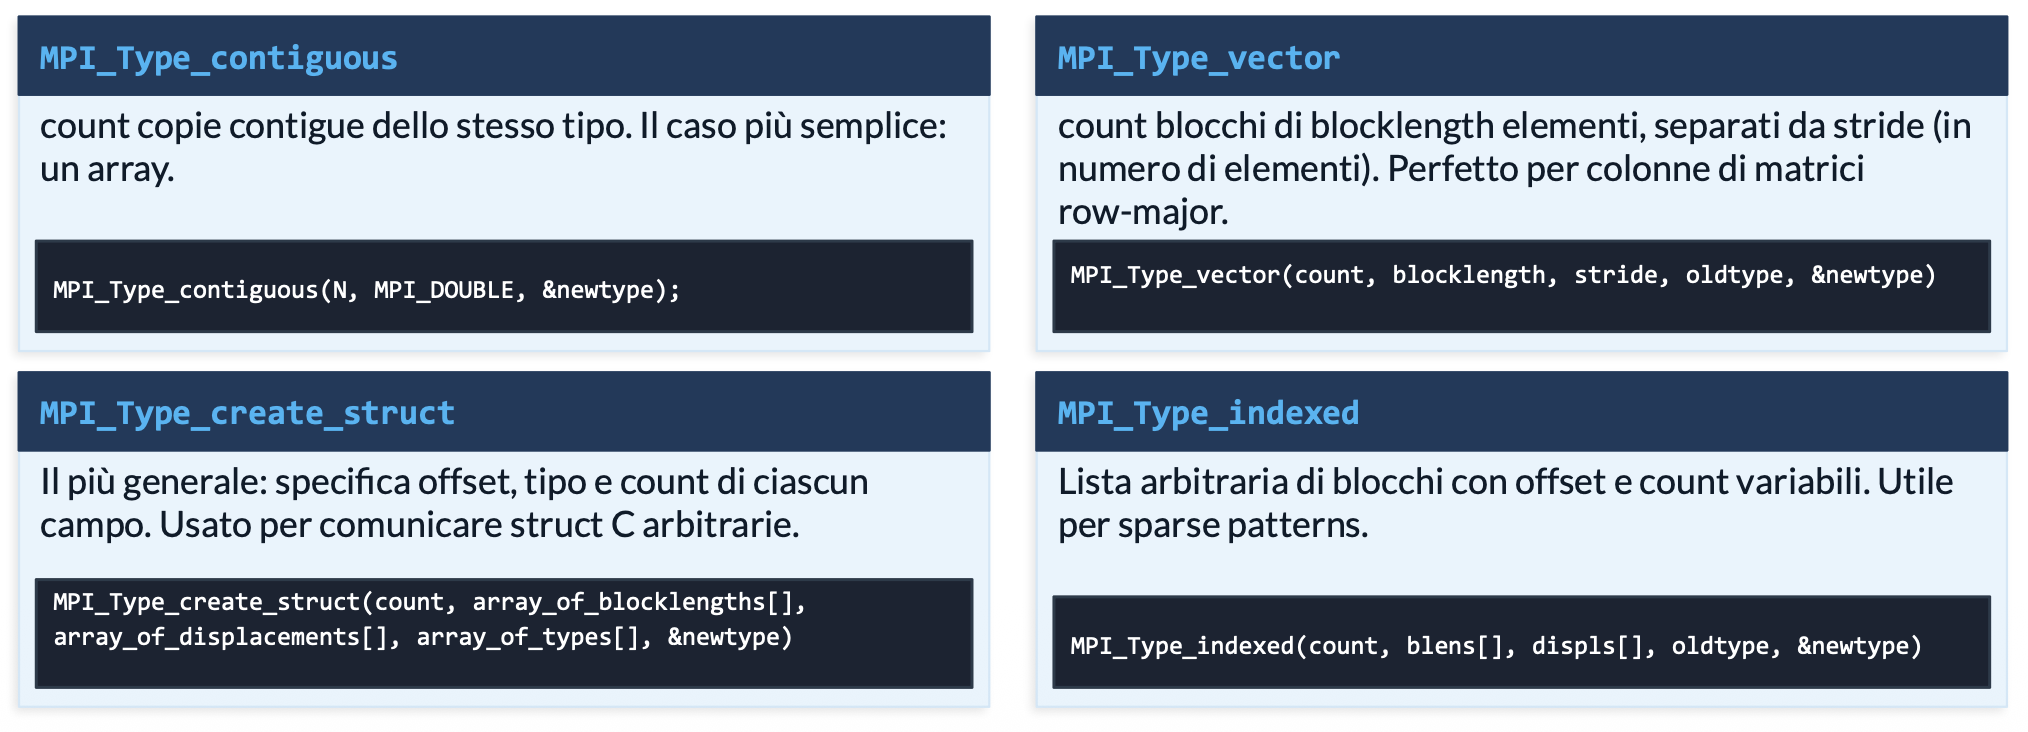
\includegraphics[width=0.9\linewidth]{Images/cap_8/derivati.png}
\end{figure}

\begin{figure}[H]
    \centering
    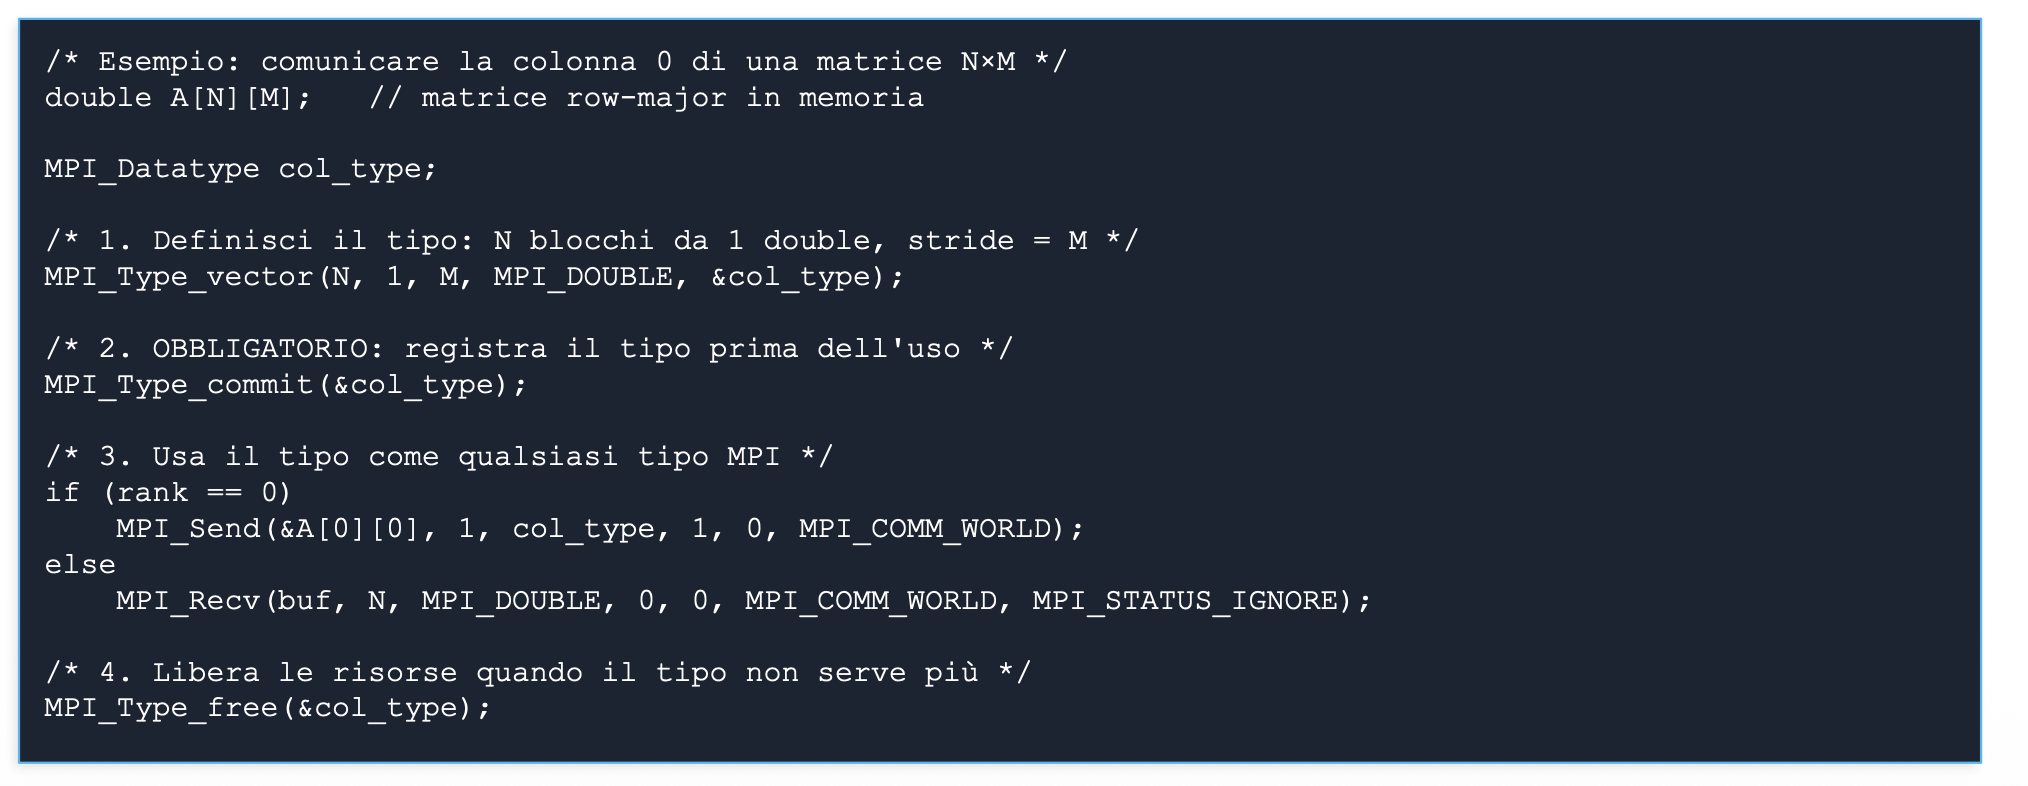
\includegraphics[width=0.9\linewidth]{Images/cap_8/workflow.png}
    \caption{Un tipo derivato deve essere registrato con MPI\_Type\_commit prima di poter essere usato nelle chiamate di comunicazione. Dopo l'uso va liberato con MPI\_Type\_free per evitare memory leak nell'implementazione MPI.}
\end{figure}

\vspace{0.5cm}
\noindent
\textbf{Anatomia di un Messaggio MPI} \\
Un messaggio è composto da due parti logiche: l'\textbf{envelope} (intestazione per il matching, cioò identifica il messaggio nel sistema) e il \textbf{data buffer} (payload effettivo).

\begin{figure}[H]
    \centering
    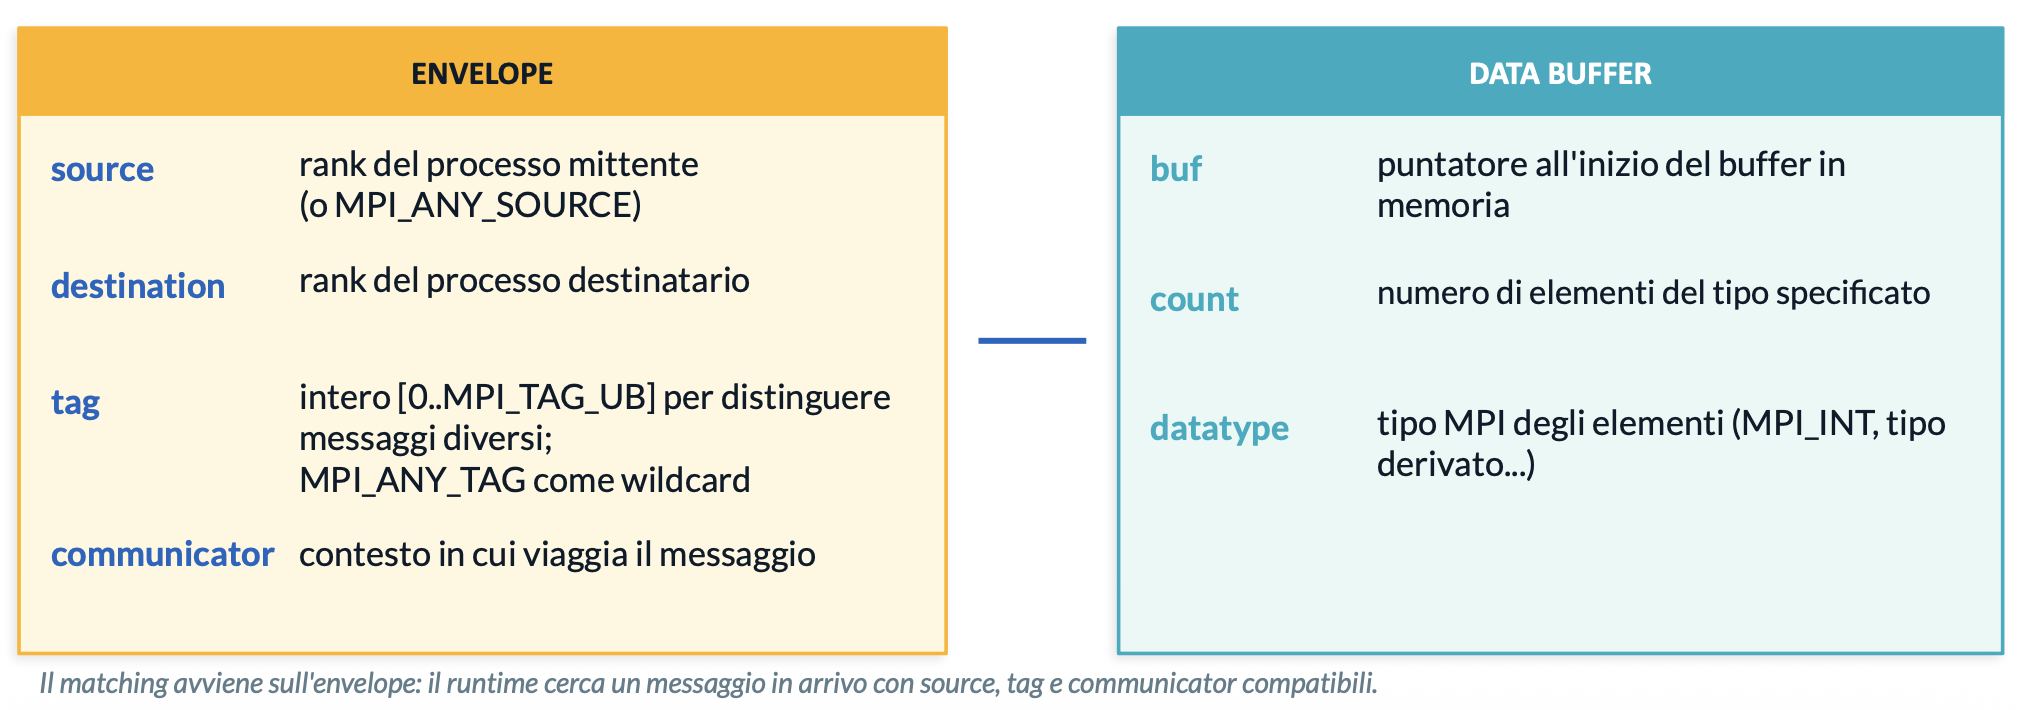
\includegraphics[width=0.8\linewidth]{Images/cap_8/anatomia.png}
\end{figure}

\section{Modalità di Comunicazione Point-to-Point}
Le funzioni fondamentali della comunicazione point-to-point sono \texttt{MPI\_Send} e \texttt{MPI\_Recv}. 

\begin{figure}[H]
    \centering
    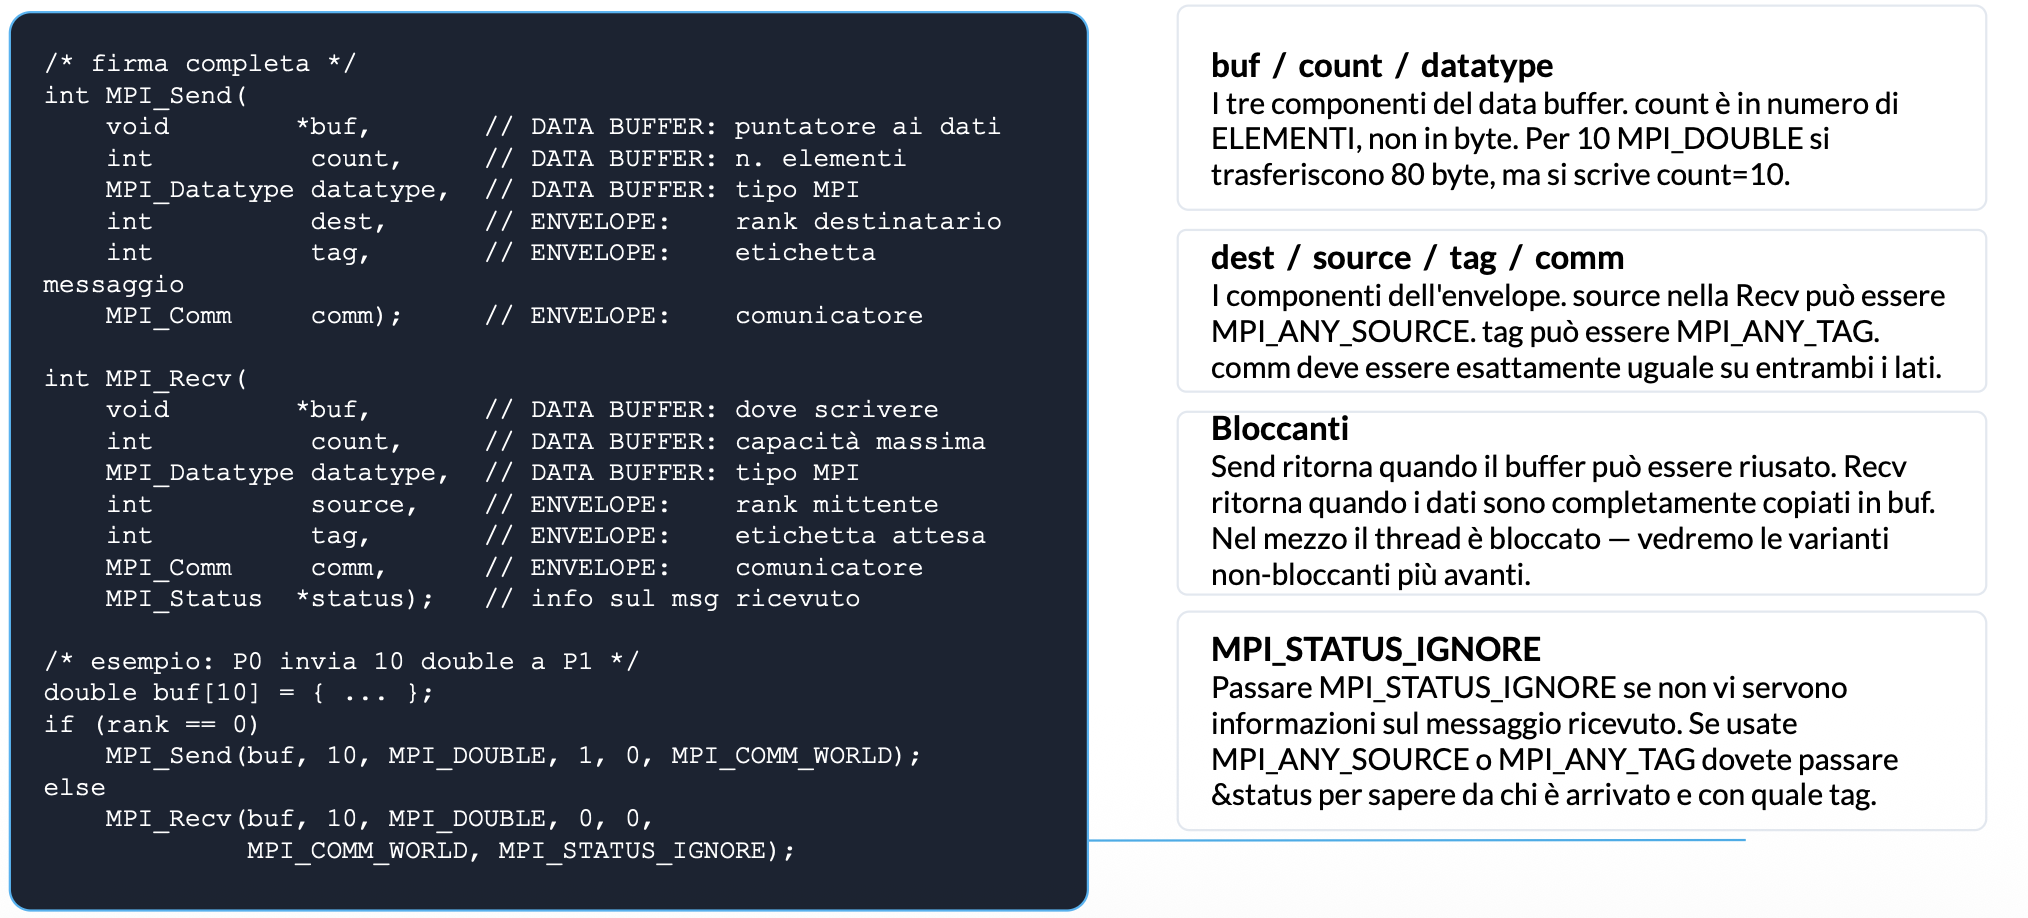
\includegraphics[width=0.8\linewidth]{Images/cap_8/send-recive.png}
\end{figure}

Esistono diverse modalità di invio con semantiche differenti. In MPI, il termine \textit{blocking} (bloccante) significa che la funzione non ritorna finché il buffer di memoria non può essere riutilizzato. Tuttavia, il modo in cui questo avviene dipende dalla modalità scelta.

\begin{description}
    \item[\textbf{Standard Mode (\texttt{MPI\_Send})}] 
    È la modalità "non deterministica". Il sistema decide autonomamente se bufferizzare il messaggio o sincronizzarsi. 
    \begin{itemize}
        \item Se bufferizzato: il mittente prosegue subito.
        \item Se non bufferizzato: il mittente attende che il destinatario sia pronto.
    \end{itemize}
    \textit{Nota: Non è sicuro assumere che il buffer sia libero immediatamente.}

    \item[\textbf{Buffered Mode (\texttt{MPI\_Bsend})}] 
    Il completamento è sempre \textbf{locale}. Il programmatore deve allocare un buffer di memoria con \texttt{MPI\_Buffer\_attach}. Una volta che i dati sono stati copiati nel buffer di sistema, la funzione ritorna. È l'unica modalità che garantisce il distacco tra mittente e ricevitore.

    \item[\textbf{Synchronous Mode (\texttt{MPI\_Ssend})}] 
    Il completamento è \textbf{remoto}. La funzione termina solo quando il processo di ricezione ha iniziato a prelevare i dati. Questo garantisce un "rendez-vous" (sincronia) tra i due processi, fondamentale per il debugging dei flussi logici.

    \item[\textbf{Ready Mode (\texttt{MPI\_Rsend})}] 
    È una modalità a "zero overhead". Si può usare solo se si ha la certezza matematica che il destinatario abbia già postato la sua \texttt{MPI\_Recv}. Se il destinatario non è pronto, l'invio fallisce silenziosamente o causa errori imprevedibili.
\end{description}

\begin{framed}
\noindent
\textbf{Il concetto di Sincronia in MPI} \\
In un sistema parallelo, meno i processi devono aspettarsi l'un l'altro, più il sistema è efficiente. Tuttavia, la sincronia fornita da \texttt{MPI\_Ssend} è spesso necessaria per evitare che il sistema esaurisca la memoria dei buffer temporanei in caso di messaggi troppo frequenti o troppo grandi.
\end{framed}

\subsection{Il problema delle Deadlock}
Supponiamo ci siano due processi che cercano di scambiarsi dei dati mediante l'uso di funzioni bloccanti come \texttt{MPI\_Send} e \texttt{MPI\_Recv}:
\begin{verbatim}
    /* Esempio di potenziale Deadlock con messaggi grandi */
    if (rank == 0) {
        MPI_Send(sbuf,N,MPI_DOUBLE,1,0,comm);
        MPI_Recv(rbuf,N,MPI_DOUBLE,1,0,comm,&st);
    } else {
        MPI_Send(sbuf,N,MPI_DOUBLE,0,0,comm);
        MPI_Recv(rbuf,N,MPI_DOUBLE,0,0,comm,&st);
    }
\end{verbatim}
Se si utilizza la classica \texttt{MPI\_Send} bloccante per scambiare messaggi di grandi dimensioni, si rischia di incappare in un \textit{deadlock} (stallo). Poiché la funzione attende che il destinatario sia pronto a ricevere il messaggio prima di sbloccarsi, entrambi i processi finiscono per fermarsi all'infinito, aspettandosi a vicenda. 

Questo problema non si presenta con i messaggi di piccole dimensioni. Implementazioni come OpenMPI, infatti, gestiscono queste situazioni avvalendosi di buffer di sistema interni: se il messaggio è piccolo, viene copiato nel buffer e la \texttt{MPI\_Send} ritorna immediatamente.

Per risolvere in modo sicuro lo scambio simmetrico di messaggi, si può utilizzare la funzione \texttt{MPI\_Sendrecv}, che garantisce che l'invio e la ricezione avvengano in modo protetto. Indipendentemente dallo stato dei buffer di sistema o dalle dimensioni (anche gigantesche) dei messaggi, il runtime di MPI orchestra internamente i flussi di dati prevenendo qualsiasi rischio di deadlock. Di questa funzione ne esistono due varianti principali:
\begin{figure}[H]
    \centering
    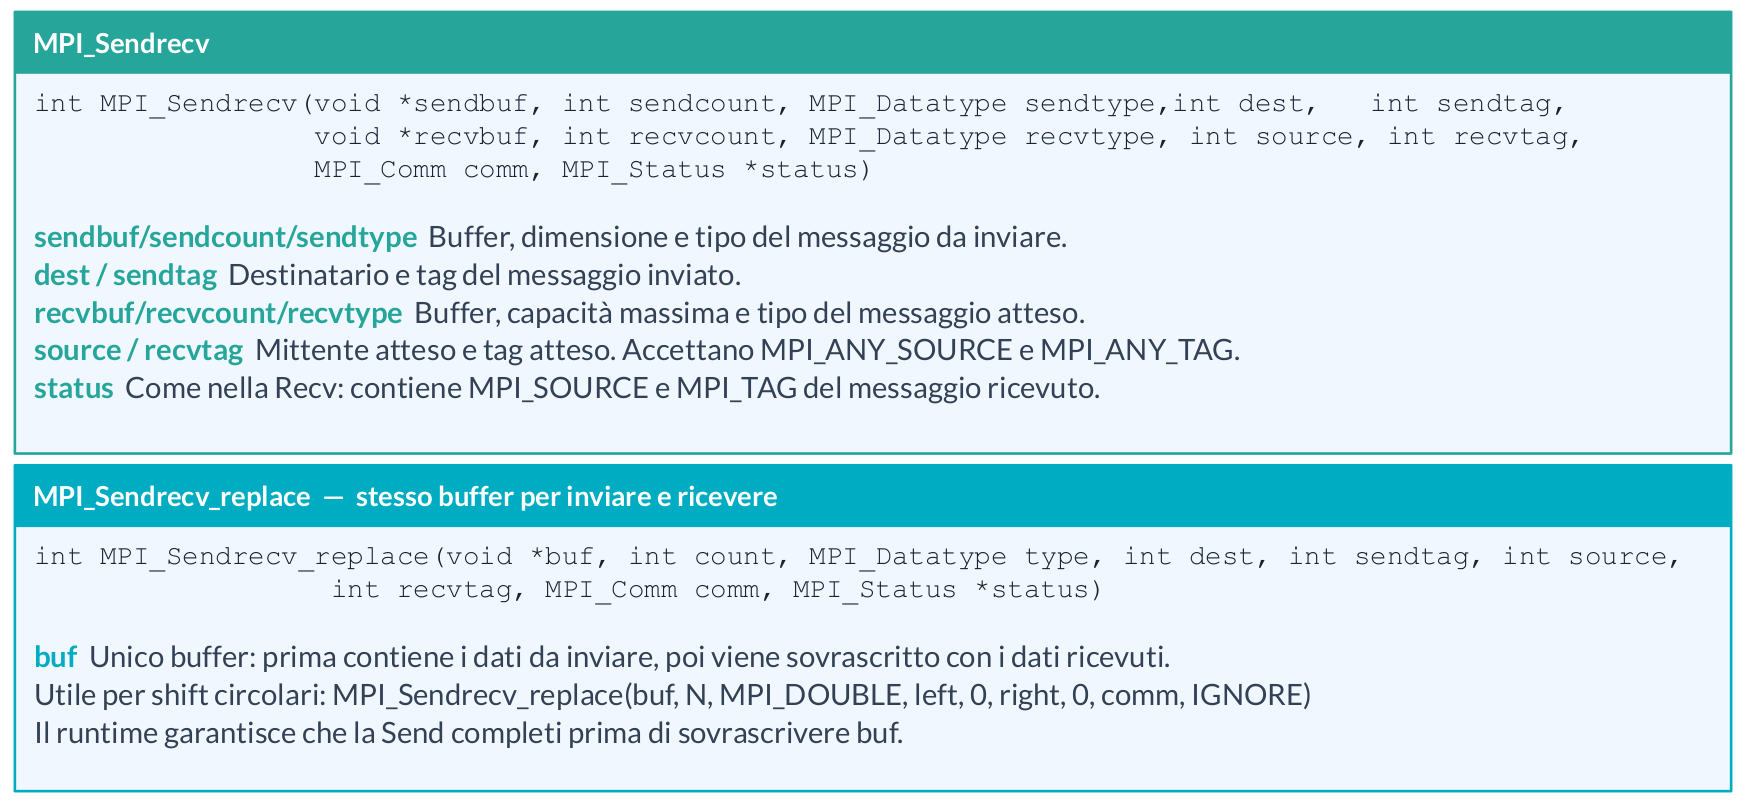
\includegraphics[width=0.7\linewidth]{Images/cap_8/mpi_send_recv.png}
\end{figure}

\subsection{Comunicazioni non bloccanti}
Il limite principale delle comunicazioni bloccanti è l'attesa inattiva: il processo si ferma in attesa che il messaggio arrivi o venga consegnato, causando rallentamenti e sprecando cicli di CPU. 

Per ovviare a questo problema si introducono le comunicazioni non bloccanti, tramite le funzioni \texttt{MPI\_Isend} e \texttt{MPI\_Irecv} (dove la \textit{I} sta per \textit{Immediate}):
\begin{figure}[H]
    \centering
    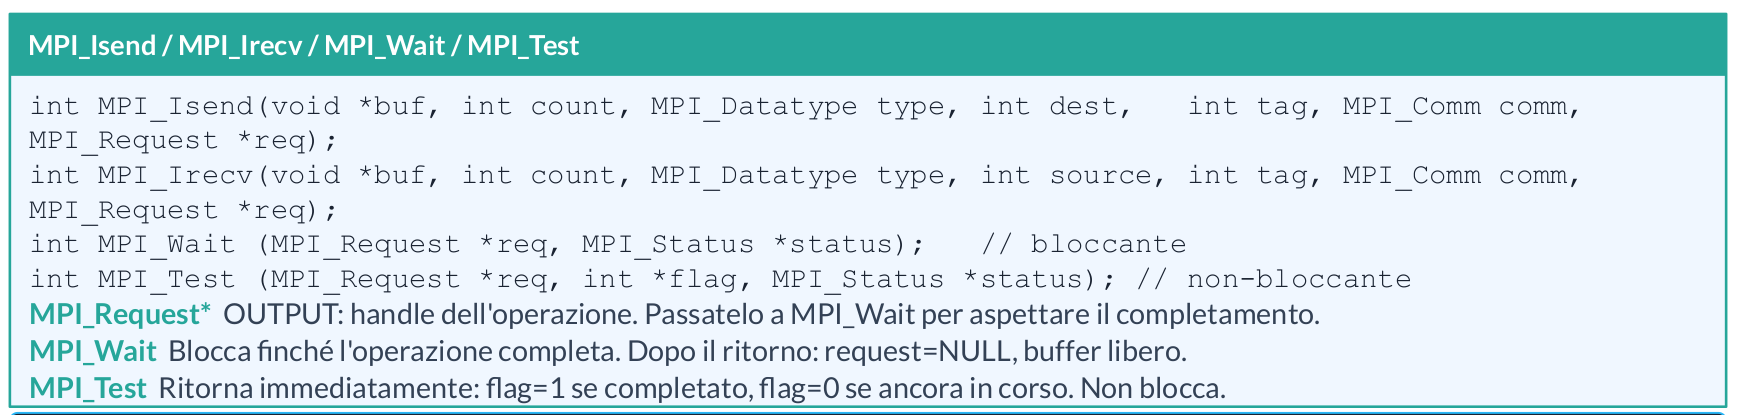
\includegraphics[width=0.7\linewidth]{Images/cap_8/isend_irecv.png}
\end{figure} 

Utilizzando queste funzioni, il processo avvia la comunicazione e riprende immediatamente l'esecuzione, permettendo di sovrapporre il trasferimento dei dati al tempo di calcolo (\textit{computation-communication overlap}). Il processo si metterà in attesa esplicita solo nel momento in cui sarà strettamente necessario utilizzare i dati ricevuti (o riutilizzare il buffer di invio). Questo si ottiene tramite la funzione \texttt{MPI\_Wait}, che forza il processo a fermarsi finché la specifica operazione non è conclusa.

È fondamentale, tuttavia, \textbf{non toccare per alcun motivo} i buffer di invio o ricezione nell'intervallo di tempo compreso tra l'avvio della chiamata asincrona e la relativa \texttt{MPI\_Wait}, poiché i dati al loro interno si trovano in uno stato inconsistente.

Il pattern corretto e tipico da applicare è il seguente:
\begin{figure}[H]
    \centering
    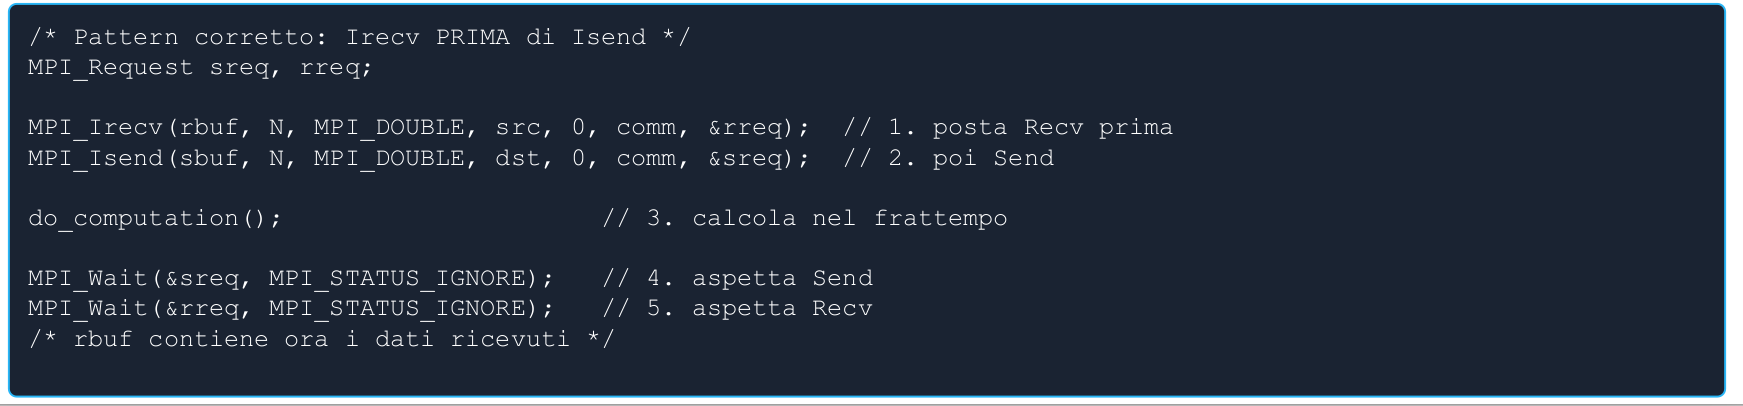
\includegraphics[width=0.7\linewidth]{Images/cap_8/pattern_isend_irecv.png}
\end{figure} 

Un'altra situazione comune è non conoscere a priori la lunghezza del messaggio in arrivo. Per gestire questa incertezza, esiste la funzione \texttt{MPI\_Probe} (e la sua variante non bloccante \texttt{MPI\_Iprobe}). Queste funzioni si limitano a ispezionare la coda dei messaggi in arrivo senza effettivamente estrarli, permettendoci di leggerne i metadati (come la dimensione) per allocare dinamicamente i buffer corretti prima di chiamare la \textit{Receive}:
\begin{figure}[H]
    \centering
    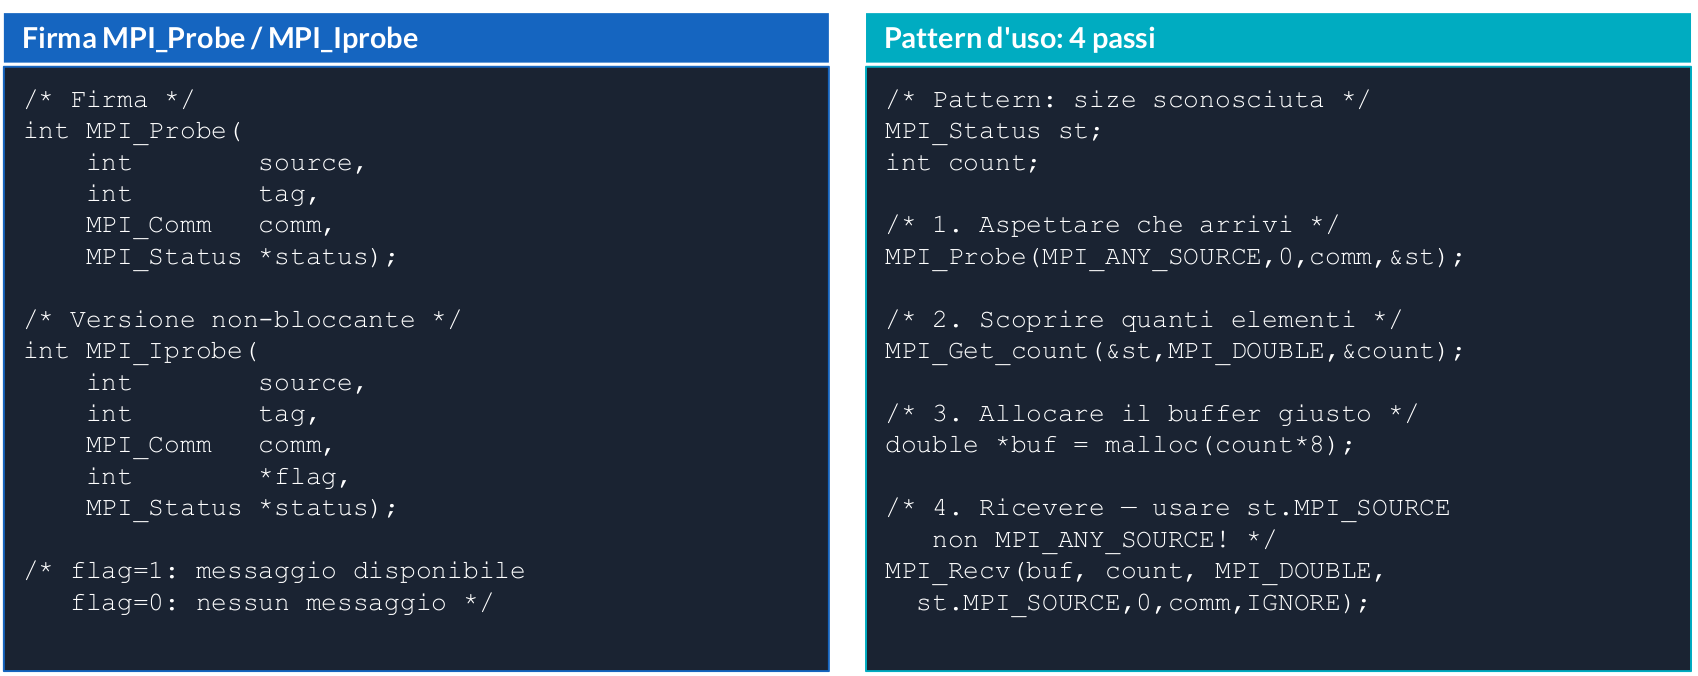
\includegraphics[width=0.7\linewidth]{Images/cap_8/pattern_firma_probe.png}
\end{figure} 

Infine, come accennato, le comunicazioni non bloccanti necessitano sempre di primitive di sincronizzazione (\textit{wait}) per garantire il corretto completamento delle operazioni ed evitare perdite di memoria. Oltre alla prima \texttt{MPI\_Wait} analizzata, esistono altre comode varianti per gestire array di richieste:
\begin{figure}[H]
    \centering
    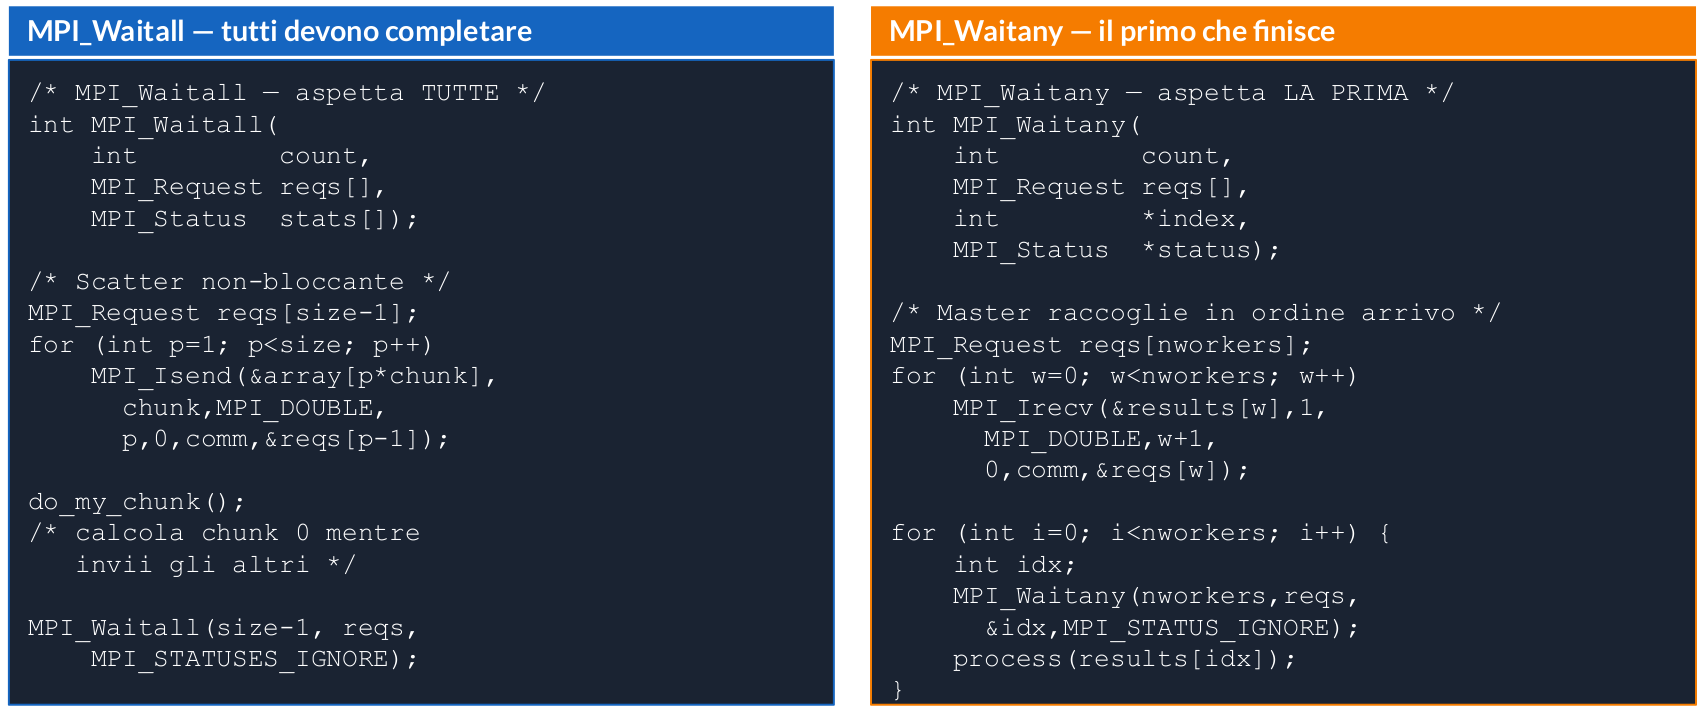
\includegraphics[width=0.7\linewidth]{Images/cap_8/waitall_waitany.png}
\end{figure}

\subsection{Linee guida per la scelta: Bloccanti vs. Non-Bloccanti}
Le funzioni non bloccanti non rappresentano sempre la scelta migliore, poiché introducono una maggiore complessità nel codice e rendono il debugging nettamente più ostico. La scelta della strategia comunicativa deve quindi basarsi su criteri pratici:

\begin{itemize}
    \item \textbf{Scegliere le funzioni BLOCCANTI quando:}
    \begin{itemize}
        \item Non ci sono computazioni utili da poter eseguire nell'intervallo tra l'invio (\texttt{MPI\_Send}) e la ricezione (\texttt{MPI\_Recv}), rendendo l'asincronia di fatto superflua.
        \item I messaggi scambiati sono di piccole dimensioni (indicativamente $< 64$~KB, al di sotto dell'\textit{eager limit}), in quanto \texttt{MPI\_Send} sfrutta la bufferizzazione interna e ritorna in modo quasi istantaneo.
        \item Si è in fase di sviluppo o debugging, poiché la semantica lineare semplifica drasticamente la riproducibilità degli errori e l'individuazione dei bug.
    \end{itemize}
    
    \item \textbf{Scegliere le funzioni NON-BLOCCANTI quando:}
    \begin{itemize}
        \item Si hanno calcoli indipendenti da eseguire contemporaneamente al tempo di comunicazione, così da nascondere i tempi morti della rete (\textit{latency hiding}), come nel caso degli algoritmi iterativi con \textit{halo exchange} o nelle computazioni \textit{stencil}.
        \item Un processo \textit{Master} deve distribuire dati a molti nodi \textit{Worker}: avviare un ciclo veloce di \texttt{MPI\_Isend} seguito da una singola \texttt{MPI\_Waitall} risulta molto più efficiente e scalabile rispetto a una sequenza bloccante di \texttt{MPI\_Send}.
    \end{itemize}
\end{itemize}

\textbf{Regola d'oro:} È sempre buona norma iniziare lo sviluppo implementando una logica lineare e robusta con le funzioni \textbf{bloccanti}. Solo successivamente si esegue la profilazione del codice (\textit{profiling}), passando alle varianti \textbf{non bloccanti} esclusivamente nei colli di bottiglia dove l'attesa di comunicazione domina nettamente sul tempo di calcolo.